\chapter{Model automobilu}
\label{sec:CarModel}
\

V této kapitole je popsán model automobilu a jeho jednotlivé součásti.

Model automobilu je založen na podvozku typu Alamak, která má \textbf{1 servomotor}
pro řízení a \textbf{2 motory} pro pohon.
\textbf{Podvozek Alamak} je řízen pomocí \textbf{NXP Freedom K66F} \cite{frdmk66UserGuide} spolu s modulem \textbf{POLI-TFC} přípojeným do GPIO pinů
MCU. Detailní popis MCU a modulu jsou v~podkapitolách \ref{sec:FRDM-K66F}
a \ref{sec:POLI-TFC}.

Pro manuální řízení je zapojen přijímač RC signálu \textbf{Minima 6S} do pinu
POLI-TFC shieldu. Přijímač pak přijímá signály z vysílače \textbf{OPTIC 6 SPORT}.

Pro komunikaci s platformou Alamak je použit \textbf{WiFi Access Point}, který je
připojen k MCU pomocí Ethernet portu. \textbf{Řádková kamera}, která je umístěna
v přední části platformy, se používá pro získání obrazu dráhy. Všechny součástky
jsou napájeny baterií typu \textbf{NiMH} o napětí 7.2~V.

Celý model je zobrazen na obrázku \ref{fig:car}.
\begin{figure}[!h]
    \centering
    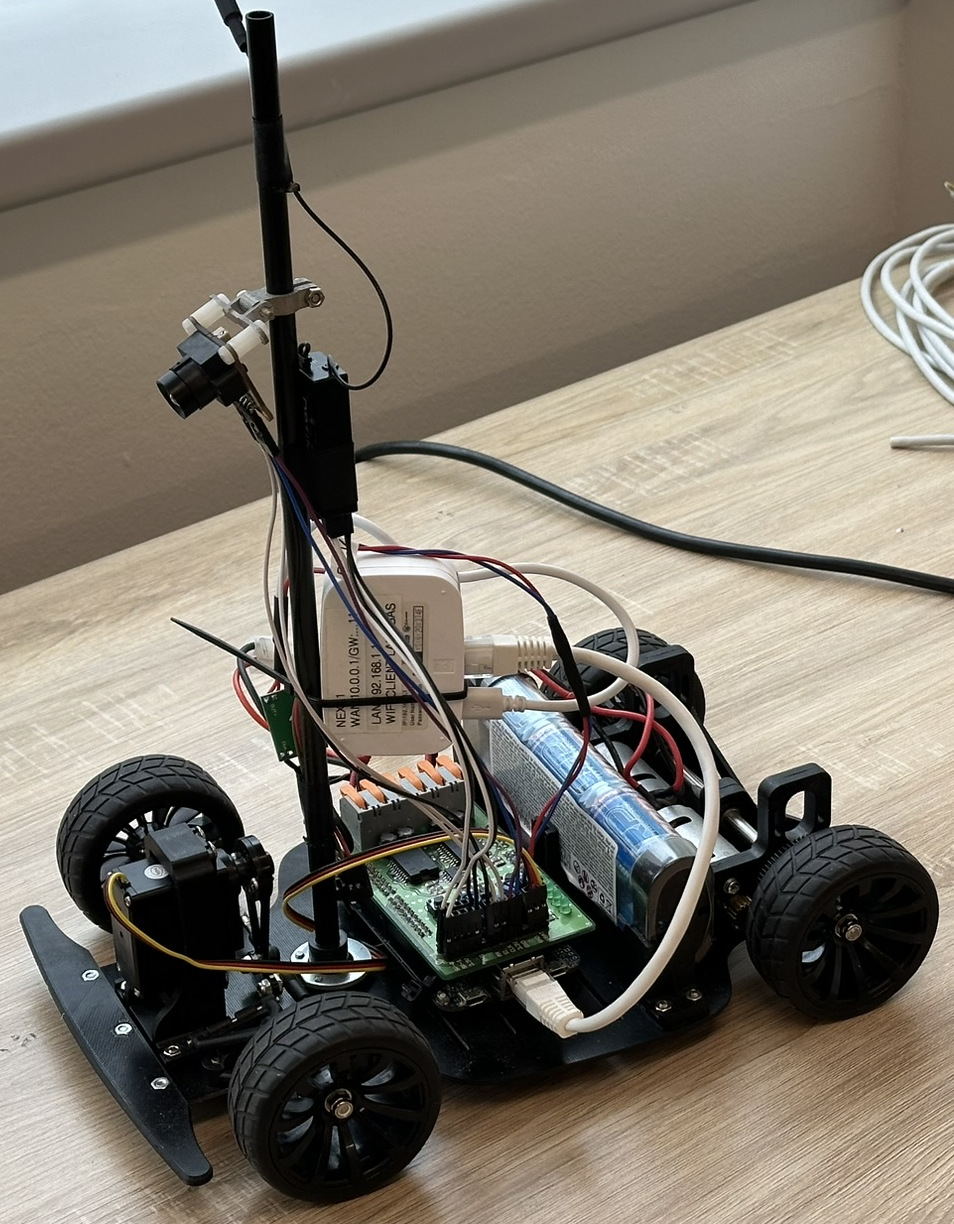
\includegraphics[width = .4\linewidth]{Figures/Car.jpeg}
    \caption{Model auta}
    \label{fig:car}
\end{figure}

\section{FRDM-K66F}
\label{sec:FRDM-K66F}\

\textbf{FRDM-K66F} je vývojová platforma od společnosti NXP určená pro MCU řady Kinetis
K66~a~K26. Platforma je založena na jádře \textbf{ARM© Cortex®-M4} a využívá model
\textbf{MK66FN2M0VMD18} s~frekvencí 180 MHz, 2 MB flash paměti a 256 KB RAM.

Konektivitu zajištují 2 micro-B USB porty, 1 ethernetový port a 54 GPIO pinů.
GPIO~piny jsou kompatibilní s \textbf{Arduino™ R3}, čímž je poskytnuta široká škála
možností pro rozšiřující desky. Deska umožňuje bezdrátové možností konektivity
pomocí modulů Bluetooth a RF.

Pro ladění je na platformě přítomno rozhraní \textbf{OpenSDAv2.1}, které podporuje
J-Link. J-Link~je sériový programovací adaptér, který umožňuje programování a
debugování mikrokontrolérů.

Další užitečné periferie na desce zahrnují trojbarevnou LED, SDHC a digitální MEMS
mikrofon.

Jako \textbf{inerciální měřicí jednotku} (IMU) platforma využívá akcelerometr
společně s magnetometrem a gyroskopem \cite{frdmk66UserGuide}.

Vývojová platforma je znázorněna na obrázku \ref{fig:FRDM-K66F}.

\section{POLI-TFC}
\label{sec:POLI-TFC}\

\textbf{POLI-TFC shield} je rozšiřující deska pro FRDM-K66F, která rozšiřuje
rozhraní pro připojení periferií k vývojové desce. Shield obsahuje 2 konektory
pro motory, 2 servomotory, 2 rozhraní pro~připojení řádkových kamer,

2 potenciometry, 4 DIP přepínače a 4 LED diody. Shield~je zobrazen na obrázku
\ref{fig:POLI-TFC}.

\begin{figure}[ht]
	\centering
	\subfloat{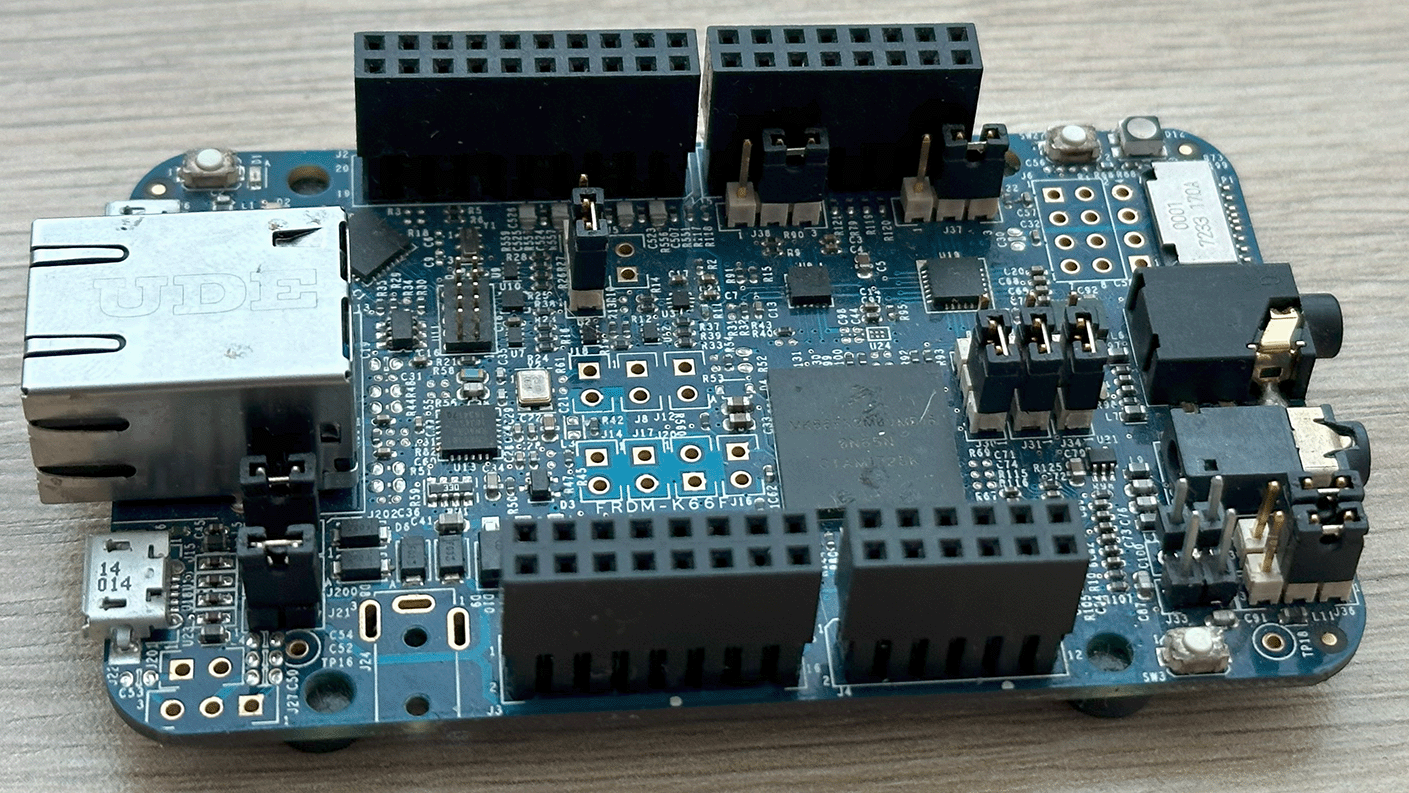
\includegraphics[width = 0.45\textwidth]{Figures/FRDM-K66F.png}\label{fig:FRDM-K66F}}
	\hfill
	\subfloat{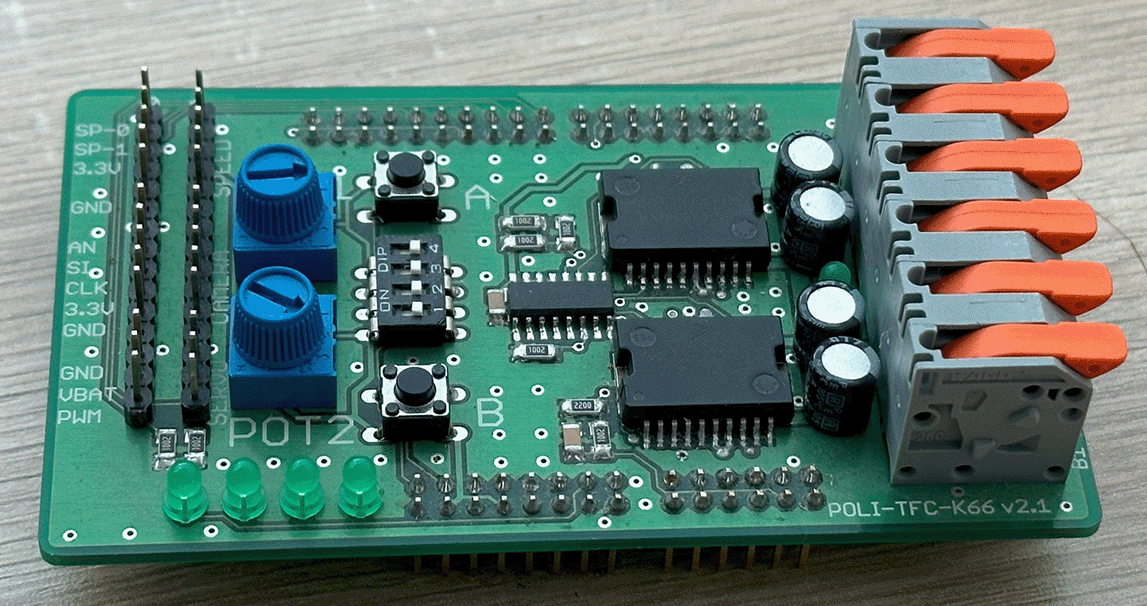
\includegraphics[width = 0.48\textwidth]{Figures/POLI-TFC.png}\label{fig:POLI-TFC}}
	\caption{Vývojová platforma FRDM-K66F (vlevo) a POLI-TFC shield (vpravo).}
\end{figure}

\endinput
